\documentclass[aspectratio=169]{beamer}
% \usetheme{Madrid}
\usepackage[%
numbering=fraction,%
block=fill,%
subsectionpage=progressbar]{pescPres}
\usepackage{caption,subcaption}
\usepackage{texmacro_maths}
\usepackage{amsthm}
 \usepackage{numprint} 
\usepackage{color, colortbl}
\definecolor{Gray}{gray}{0.9}
\usepackage{graphicx}
\usepackage[export]{adjustbox}
\usepackage{outlines}
%\renewcommand{\arraystretch}{0.4}% Tighter
% \DeclareMathOperator*{\argmax}{arg\,max}
% \DeclareMathOperator*{\argmin}{arg\,min}
\usepackage{biblatex}
%\addbibresource{example.bib}
%\bibliography{example}

\setlength{\intextsep}{1cm}

\title{Agrupando Redes com Atributos usando as Divergências de Bregman}

\author{Felipe Schreiber Fernandes \\
    [1em]{Orientadores: \\
    \text{\hspace{2em}Daniel Ratton Figueiredo (UFRJ)}\\
    \text{\hspace{2em} Maximilien Dreveton (EPFL, Suíça)}}
}

\renewcommand{\arraystretch}{0.9}
\begin{document}
     \maketitle
     \begin{frame}{Clusterização}
     	\begin{itemize}
     		\item Metodo para agrupar dados com similaridade. 
     		\item Problema estudado há mais de 40 anos (Kmeans 1956)
     			\item Como encontrar agrupamentos? 
     			\begin{figure}
     				\centering
     				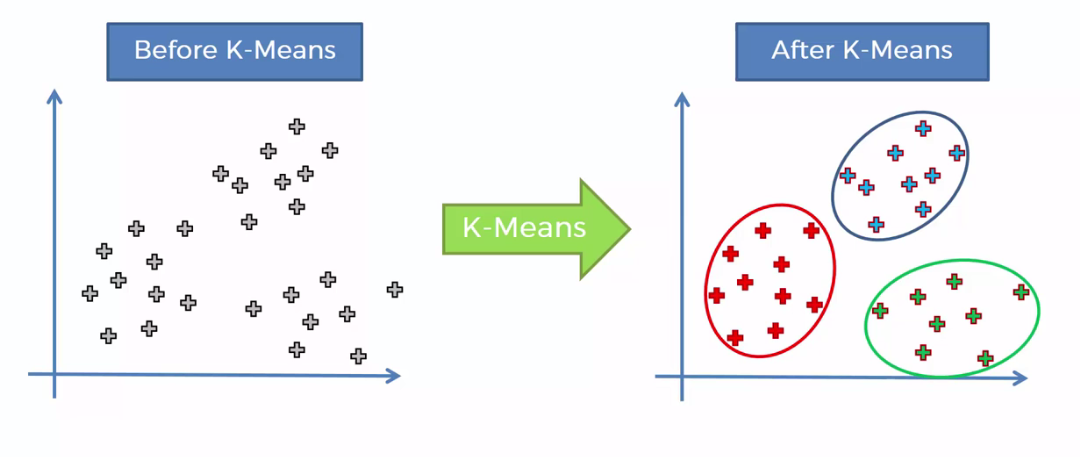
\includegraphics[scale=0.15]{img/kmeans.png}
     			\end{figure}
     			\item E se tivéssemos um grafo? (Louvain 2008)
     			\begin{figure}
     				\centering
     				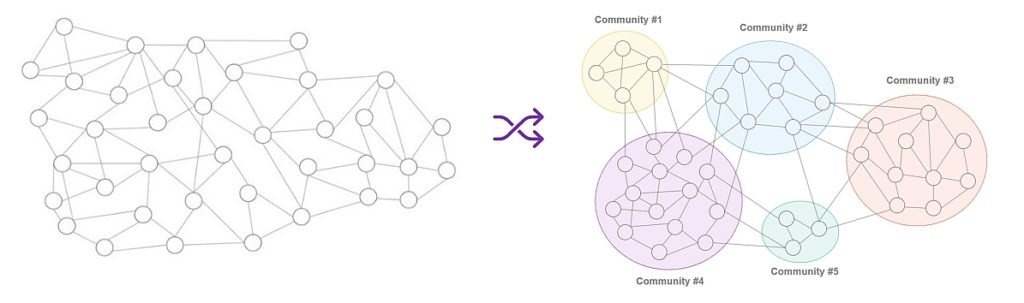
\includegraphics[scale=0.15]{img/louvain.jpg}
     			\end{figure}
     	\end{itemize}
     \end{frame}
     
     \begin{frame}{Clusterização de Redes}
		\begin{figure}
			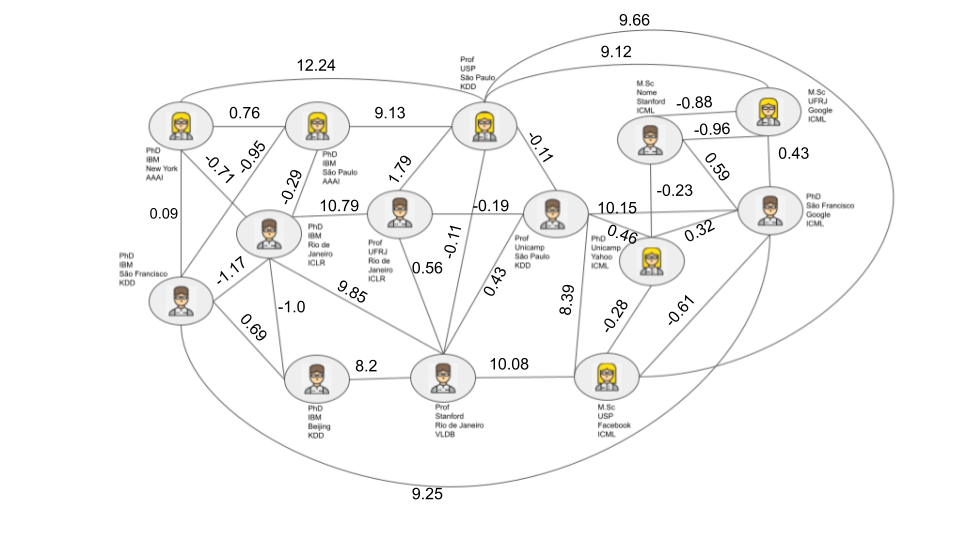
\includegraphics[scale=0.3]{img/Imagens_CTD_before.png}
			\caption{Rede de citações}
			\label{fig:imagensctdbefore}
		\end{figure}
     \end{frame}
          \begin{frame}{Clusterização de Redes}
     	\begin{figure}
     		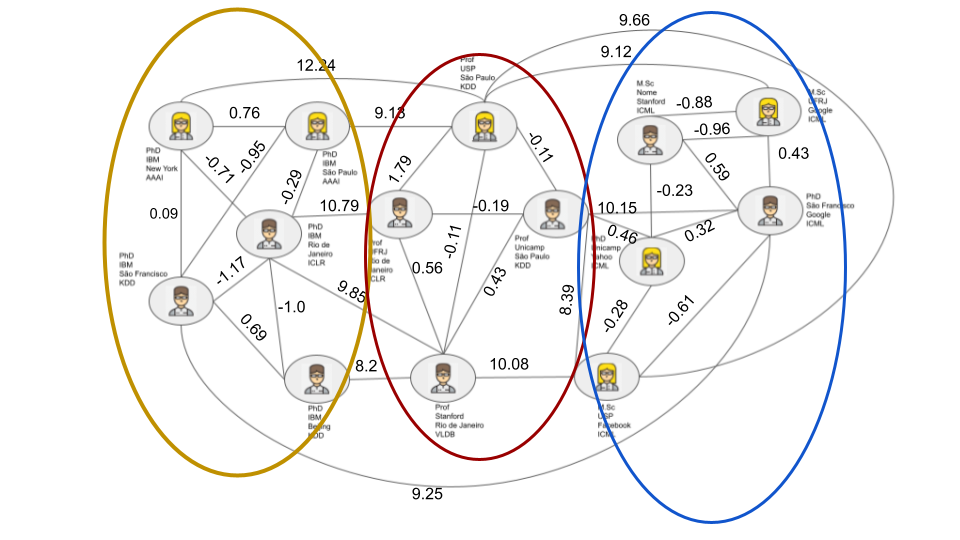
\includegraphics[scale=0.3]{img/Imagens_CTD_after.png}
     		\caption{Rede de citações}
     		\label{fig:imagensctdafter}
     	\end{figure}
     \end{frame}
     
\begin{frame}{Nossa contribuição}
    \begin{itemize}
    	\item Modelo matemático para redes esparsas com atributos
    	\item Algoritmos baseados em inferência estatística para obter o agrupamento
        \item Novos métodos de inicialização
        \item Avaliação e comparação do algoritmo em redes sintéticas e reais
    \end{itemize}
\end{frame}

% \begin{frame}{Bregman Divergences}
% \begin{minipage}{0.45\textwidth}
%     \begin{itemize}
%         \item A divergence D is a function that measures the dissimilarity between two points P and Q in a manifold. 
%         \item In general $D[P,Q] \neq D[Q,P]$, so it can't be interpreted as a distance.
%         \item Non-negativity: $D[P,Q] \geq 0$
%         \item $D[P,Q] = 0 \iff P = Q$
%     \end{itemize}
% \end{minipage}
% \begin{minipage}{0.45\textwidth}

%     \begin{itemize}
%         \item The Bregman Divergences have following form: 
%             \begin{align*}
%                 D[P,Q] = \psi(P) -  \psi(Q) - \nabla\psi(Q)(P - Q)
%             \end{align*}
%         \item Convexity with respect to the first argument.
%         \item Each exponential distribution is related to a unique dual pair ($\psi,\phi$).
%     \end{itemize}
% \end{minipage}
% \end{frame}

% \begin{frame}{Bregman Divergences and exponential family}
%  \hspace{1cm} The form of exponential distributions is given by:
%     \begin{equation*}
%     p_{\psi,\theta} = p(x, \theta) = \exp\{\theta h(x) + k(x) - \psi(\theta)\}
%     \end{equation*}
% \begin{itemize}
%     \item x is a random variable
%     \item h(x) are linear independent functions of x (sufficient statistics)
%     \item $\psi$ is a potential function that $\int_\Omega p_\theta(x)dx = 1$ $\psi(\theta) = \log \int_\Omega \exp{k(x) + \theta h(x)} dx$
%     \item Forster and Warmuth established that $p_{\psi,\theta} = p_{\phi,\mu}  = \exp\{-d_\phi(x, \mu)\}b_\phi(x)$
%     \item The dual parameters are normally expressed as:
%     \begin{align*}
%          \mu(\theta) = \nabla\psi(\theta),
%          \theta(\mu) = \nabla\phi(\mu)
%     \end{align*}
% \end{itemize}
% \end{frame}

% \begin{frame}{Example of distribution}
%     % \begin{figure}[h]
%     % \centering\includegraphics[scale=0.4]{img/exponential_dsitributions.png}
%     % \end{figure}
% \begin{minipage}{0.9\textwidth}
%        \hspace{1cm} Let's take for example the Gaussian distribution with unit variance. We can write as follows:
% \begin{align*}
%     p(x,a) = \frac{1}{\sqrt{(2\pi\sigma)^d}}\exp{\{\frac{-1}{2\sigma^2}||x-a||^2\} }\\
%     p(x,\theta) = \exp {\{\langle x,\theta \rangle - \psi(\theta)\}}b(x)
% \end{align*}
% The second expression is in the canonical form $p(x,\theta) = \exp\{\langle\theta, h(x)\rangle - \psi(\theta)\}p(x)$ with:
% {\small
% \begin{align*}
%     \theta = \frac{a}{\sigma^2},\quad
%     \psi(\theta) = \frac{\sigma^2||\theta||^2}{2},\quad \phi(\mu) = \frac{||\mu||^2}{2\sigma^2}\\
%     p(x) = \exp{\{\frac{-1}{2\sigma^2}||x||^2\} }\frac{1}{\sqrt{(2\pi\sigma)^d}}, \quad d_\phi(x,\mu) = \frac{(x-\mu)^2}{2\sigma^2}
% \end{align*}
% }%
% \end{minipage}
 
% \end{frame}

%\begin{frame}{Agrupando com as Divergências de Bregman 
%	\footnote{ Banerjee et al. Clustering with Bregman Divergences - JMLR}
%}
%\begin{minipage}{0.9\textwidth}
%    \begin{itemize}
%        \item A função objetivo é definida como:
%        \begin{equation*}
%            J_\phi(s) = \min_{s \in R^d}E_p[d_\phi(X,s)] 
%        \end{equation*}
%        \item $s^* = \mu = E_p[X]$
%        \item $X,s \in R^d$
%    \end{itemize}
    % \begin{proof}
    % {\small
    %     \begin{align*}
    %         J_\phi(s) - J_\phi(\mu) = E_p[d_\phi(X,s)] - E_p[d_\phi(X,\mu)])\\
    %         = \phi(\mu)-\phi(s)-\langle\nabla\phi(s),\mu-s\rangle\\
    %         = d_\phi(\mu,s) \geq 0 
    %     \end{align*}
    % }%
    % \end{proof}
%\end{minipage}
% \begin{minipage}{0.45\textwidth}
%     \begin{itemize}
%         \item For the soft clustering, we have:
%         {\small
%         \begin{align*}
%             L(M) = P(x|M) = \sum_{j=1}^K\pi_jexp\{-d\phi(x, \mu)\}b_\phi(x)
%         \end{align*}
%         }%
%         \item \textbf{E-step}:
%         {\small
%             \begin{align*}
%             p(x_i \in C_j) = \frac{ \pi_jexp\{-d\phi(x, \mu_j)\}b_\phi(x)}{ \sum_{h=1}^K\pi_h exp\{-d\phi(x, \mu_h)\}b_\phi(x)}
%             \end{align*}
%         }%
%         \item \textbf{M-step}:
%         {\small
%             \begin{align*}
%                 \pi_j = \frac{1}{N}\sum_ip(x_i \in C_j),
%                 \mu_j = \frac{\sum_ip(x_i \in C_j)x_i}{{\sum_{i=1}^N p(x_i \in C_j)}}
%             \end{align*}
%         }%
%     \end{itemize}
% \end{minipage}
%\end{frame}

% \begin{frame}{Clustering with Bregman Divergences (cont.)}
% \begin{figure}
%     \centering
%     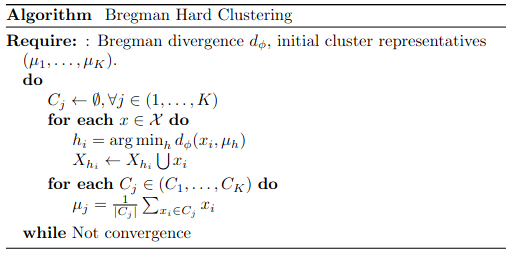
\includegraphics[scale=0.6]{img/hard_breg.png}
% \end{figure}
% \end{frame}

% \begin{frame}{Clustering with Bregman Divergences (cont.)}
% \begin{figure}
%     \centering
%     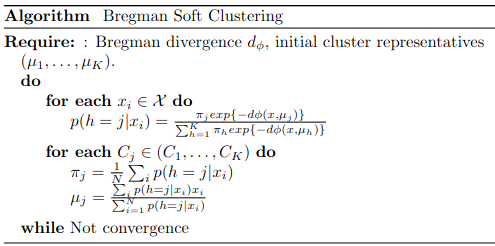
\includegraphics[scale=0.6]{img/soft_breg.png}
% \end{figure}
% \end{frame}

%
%DIVIDIR O SLIDE EM 2:
%- O PRIMEIRO: explicando os parametros do modelo distribuição de pesos e arestas para cada par (DAR EXEMPLO)
%
%- O SEGUNDO: Falar do modelo matemático, de forma geral. Dar a mesma rede do slide anterior. Perguntar "qual a probabilidade de gerar essa rede dado um conjunto de labels?" mostrar a eq.

\begin{frame}{Modelo proposto}
    \begin{outline}
    	\1 Assumimos a independência condicional entre atributos e rede
%    	\footnote{ $\mathbb{P} \left( X,Y | z \right) = \mathbb{P}\left( X | z \right)\mathbb{P}\left( Y | z \right) $}
    	\1 Para a geração dos dados:
    		\2 Gerar os atributos dos vértices $\mathbb{P}\left( Y | z \right) = \mathbb{P}\left( Y | z, \nu \right)$
    		\2 Gerar as arestas e pesos da rede $\mathbb{P}\left( X | z \right) = \mathbb{P}\left( X | z, p, \mu \right)$
      
    \end{outline}
    \begin{minipage}[t]{.35\columnwidth}
    	\begin{figure}
			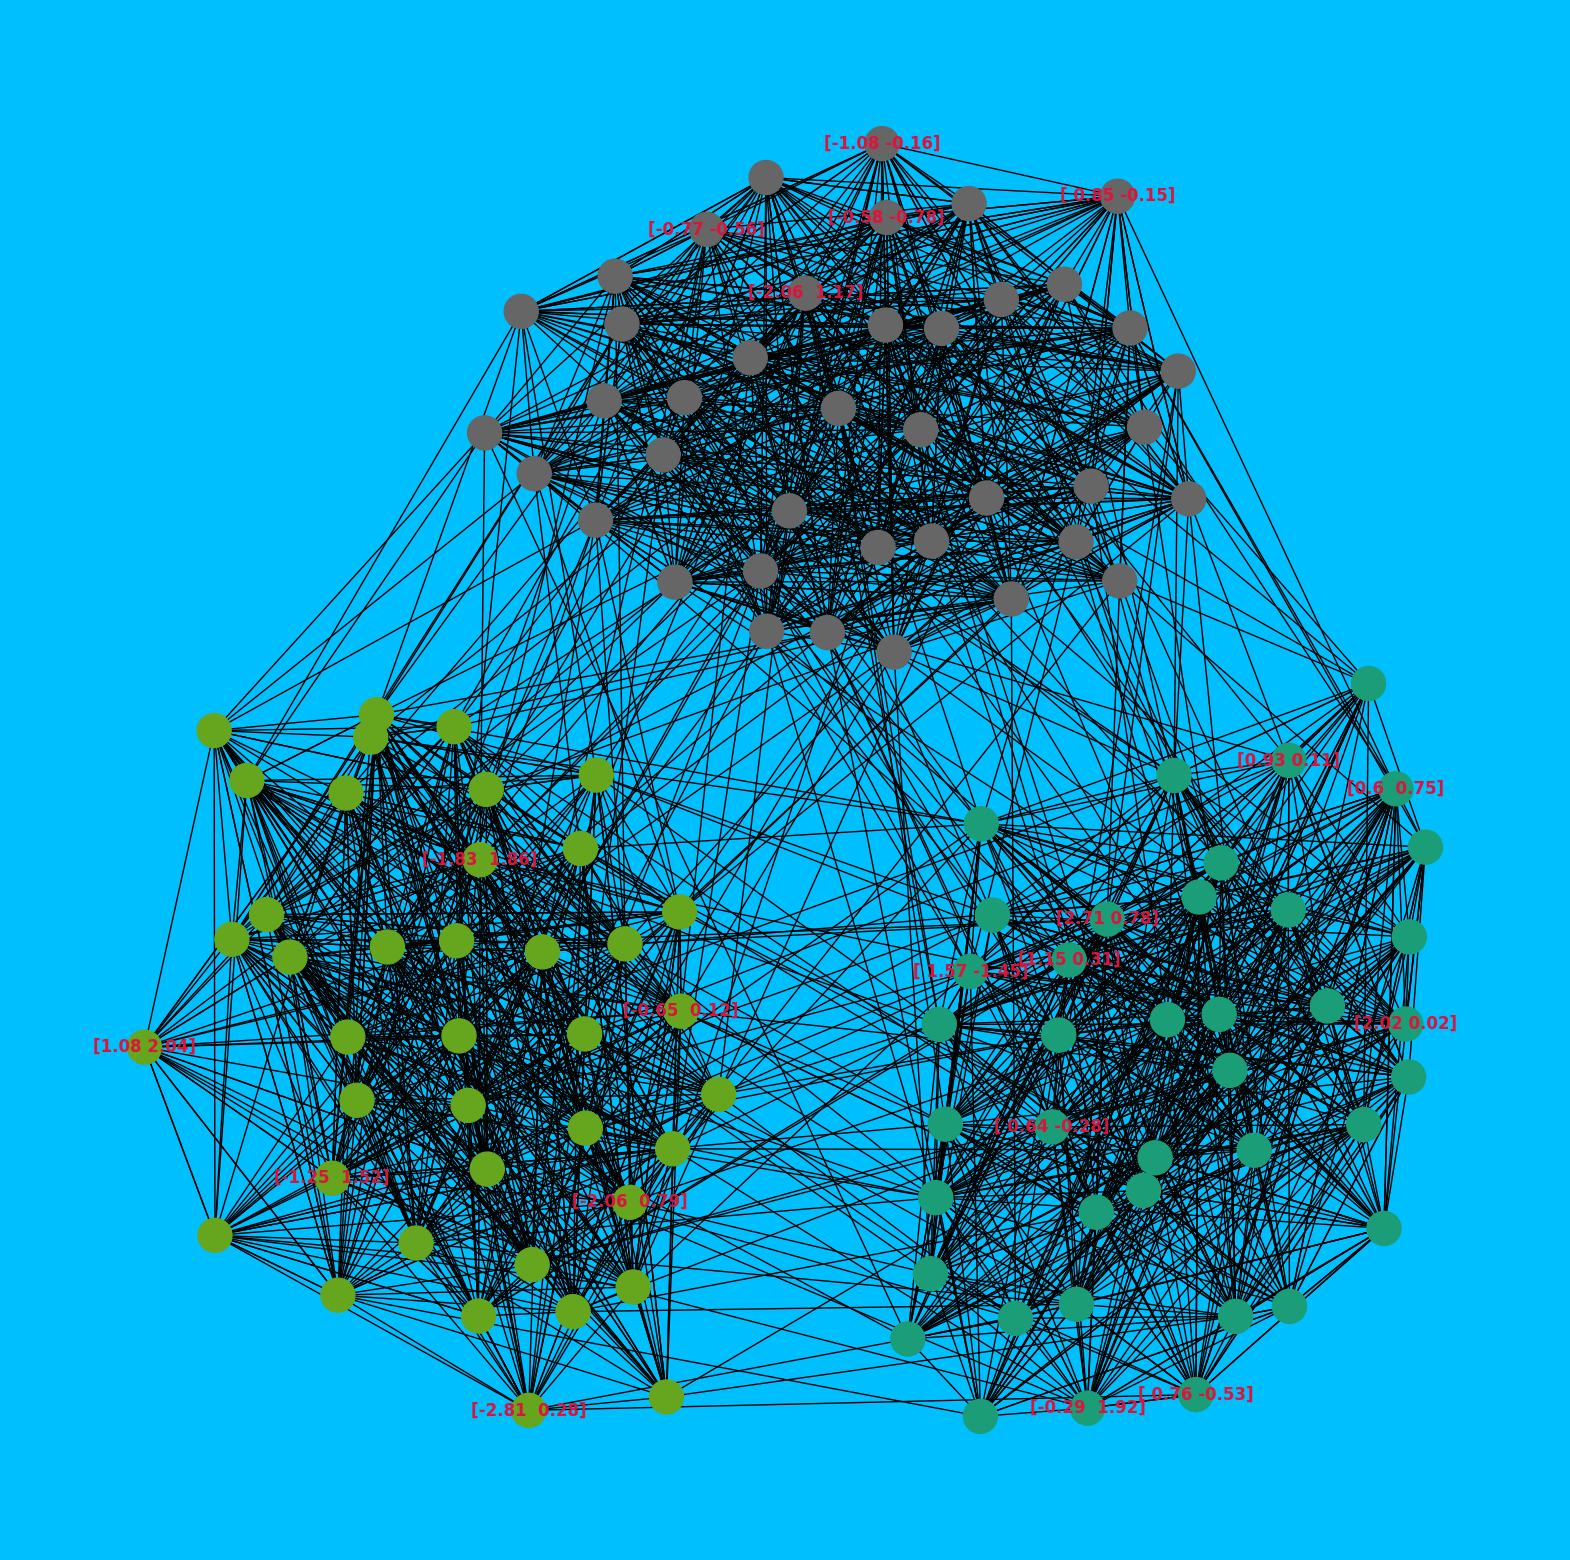
\includegraphics[scale=0.08,valign=t,width = 4cm]{img/network_example.png}
			\caption{Exemplo de grafo gerado com atributos e redes condicionalmente independentes}
		\end{figure}
    				
    \end{minipage}
%\hfill
	\begin{minipage}[t]{.35\columnwidth}
	
\[
		P =
		\begin{bmatrix}
			0.4 & 0.02 &  0.02\\
			0.02 & 0.4 & 0.02 \\
			0.02 & 0.02 & 0.4
		\end{bmatrix}
		\]
\[
		\nu = 
		\begin{Bmatrix}
			1. & 0.\\
			-0.5 & 0.86\\
			-0.5 & -0.86
		\end{Bmatrix}
\]

    \end{minipage}
    	\begin{minipage}[t]{.25\columnwidth}
    		\[
    		\mu =
    		\begin{bmatrix}
    			10 & 9 &  9\\
    			9 & 10 & 9 \\
    			9 & 9 & 10
    		\end{bmatrix}
    		\]
    	\end{minipage}
\end{frame}


\begin{frame}{Modelo proposto (Cont.)}
	\begin{minipage}{0.65\columnwidth}
	\begin{outline}
		\1 A verossimilhança tem a seguinte forma:
		\begin{align*}
			\mathbb{P} \left( X,Y | z \right) = \prod_{ 1\le i < j \le n } f_{z_i z_j}( X_{ij}) \prod_{i=1}^n h_{z_i} (Y_i)
		\end{align*}
		\1  $f_{k\ell}(x)$ denota a probabilidade de dois vértices em blocos $k$ e $l$ possuírem uma relação $x \in X$. 
		\footnote{$f_{kl}(x) = (1-p_{kl}) \delta_0(x) + p_{kl} \fpos_{kl}(x)$}
		\1 $h_k(y)$ denota a probabilidade de um vértice no bloco $k \in [K]$ possuir um atributo $y \in Y$.
		\1 Z é um vetor contendo as classes para cada vértice		
	\end{outline}
\end{minipage}
\begin{minipage}{0.32\columnwidth}
A log-likelihood da densidade $p_{\psi, \theta}$ de uma distribuição da família exponencial se relaciona com a divergência de Bregman por:
%(see for example~\cite[Equation~13]{banerjee2005clustering}) 
\begin{equation*}
	\log p_{\psi, \theta}(x) \weq - d_{\psi^*}(x, \mu ) + \psi^*(x),
\end{equation*}
onde $\mu = \E_{p_{\psi, \theta}} (X)$ é a média da distribuição.
\end{minipage}
%\begin{minipage}{0.3\columnwidth}
%	\begin{figure}
%		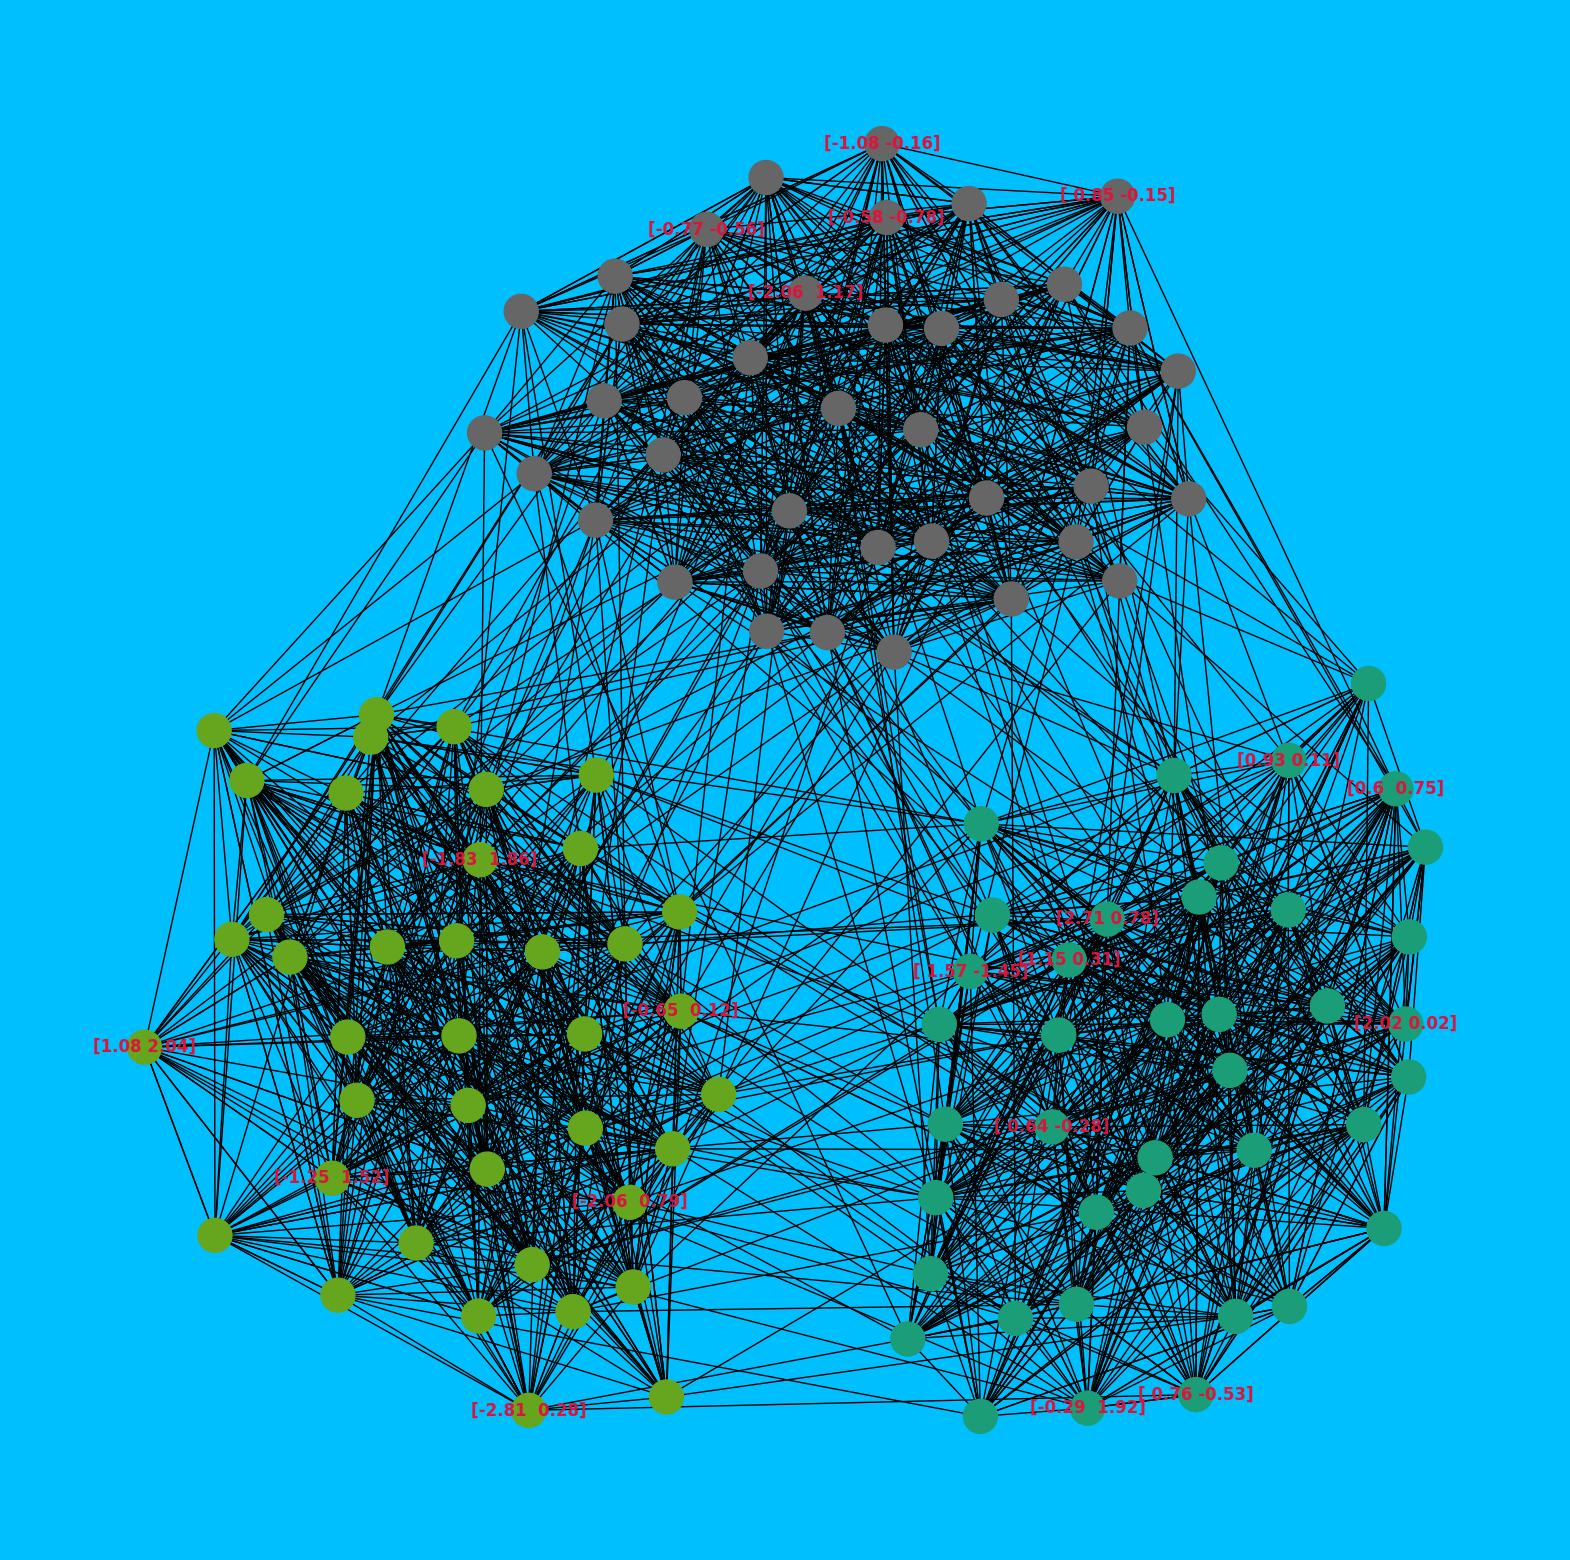
\includegraphics[valign=t,scale=0.02]{img/network_example.png}
%	\end{figure}
%	Qual a probabilidade de gerarmos o grafo anterior dado que x\% dos vértices estão corretos? 
%	\begin{itemize}
%		\item x = 100\% $\propto exp(-15469)$
%		\item x = 80\% $\propto exp(-24581)$
%		\item x = 50\% $\propto exp(-35916)$
%	\end{itemize}
%\end{minipage}
\end{frame}


%% ENCONTRAR A MELHOR COMUNIDADE PARA CADA VÉRTICE DADO: PARAMETROS E AS COMUNIDADES DOS DEMAIS

%% A CADA ITERAÇÃO OS VERTICES PODEM MUDAR DE COMUNIDADE POIS AS COMUNIDADES DOS VIZINHOS MUDAM

%% PODE CHEGAR NUM PONTO FIXO, EM QUE OS LABELS NÃO MUDAM, OU CHEGAR NO NUMERO MAX DE ITERAÇÕES
\begin{frame}{Hard Clustering}
	\begin{figure}
		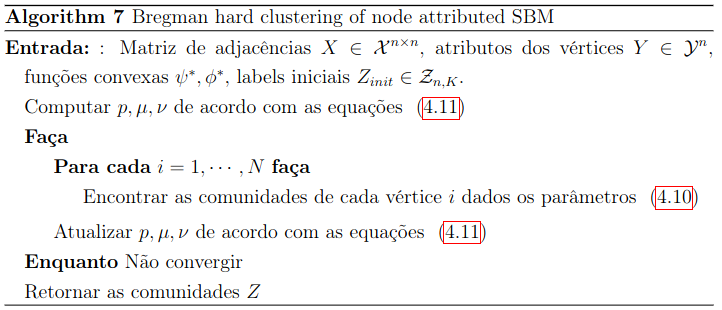
\includegraphics[scale=0.45]{img/HardBregmanSBM.png}
	\end{figure}
\end{frame}



\begin{frame}{Inicialização}
	\begin{itemize}
		\item Alternativa 1:
			Utilizar ou a rede ou os atributos
			\begin{figure}
				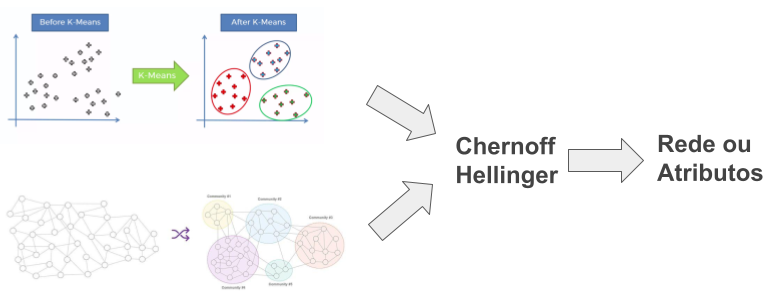
\includegraphics[scale=0.25]{img/InitProcedures.png}
			\end{figure}
		\item Alternativa 2:
			Utilizar ambas as fontes de informação
		\begin{figure}
			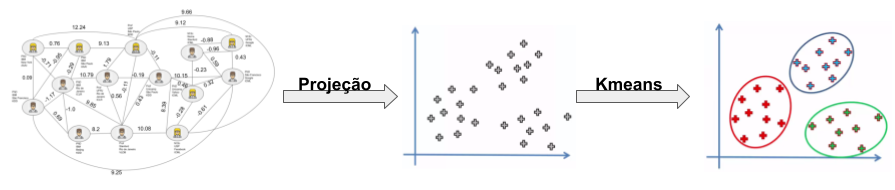
\includegraphics[scale=0.4]{img/SpectralClustering.png}
%			\caption{SpectralClustering}
%			\label{fig:spectralclustering}
		\end{figure}
	\end{itemize}
\end{frame}

\begin{frame}{Avaliação}
%PRECISAMOS SABER O GROUNDTRUTH PARA COMPARAR. Quanto maior R, mais fácil de encontrar as comunidades.
%Quanto maior a, mais fácil vai ser de separar a rede.
\begin{itemize}
\item Precisamos avaliar e comparar algoritmos em diferentes cenários.
\end{itemize}

\begin{minipage}{0.45\textwidth}
Atributos
\begin{itemize}
    \item Especificar os centros das distribuições sobre um círculo de raio R
\end{itemize}
    \begin{figure}
        \centering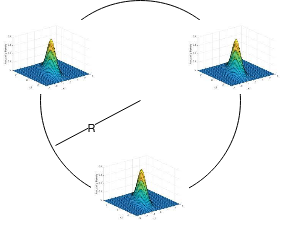
\includegraphics[scale=0.4]{img/synthetic_net.png}
    \end{figure}
\end{minipage}
\hfill
\begin{minipage}{0.45\textwidth}
Rede
\begin{itemize}
    \item Obter a rede pelo modelo SBM. $p_{in} = a\frac{\log n}{n}$, $p_{out} = b\frac{\log n}{n}$
    \item Especificar os pesos da rede $w_{in}$ e $w_{out}$
\end{itemize}
\begin{figure}
    \centering
    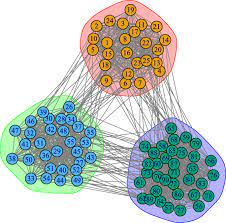
\includegraphics[scale=0.3]{img/SBM_.jpeg}
\end{figure}
\end{minipage}
\end{frame}

\begin{frame}{Comparação de Algoritmos}
    \begin{itemize}
        \item Apenas atributos - GMM (Modelo de Mistura Gaussiana)
        \item Apenas a rede - Leiden
        \item Hard clustering com ambas as fontes de informação e Divergências de Bregman
        \item Soft clustering com ambas as fontes de informação e Divergências de Bregman
        \item Attributed Stochastic Block Model \footnote{STANLEY, N., BONACCI, T., KWITT, R., et al. “Stochastic Block Models
        	with Multiple Continuous Attributes” - Applied Network Science 2019}
        \item Contextual Stochastic Block Model (IR\_sLS) \footnote{BRAUN, G., TYAGI, H., BIERNACKI, C. “An iterative clustering algorithm for the Contextual Stochastic Block Model with optimality guarantees” - ICML 2022}
    \end{itemize}
\end{frame}

\begin{frame}{Resultados}
%	FALAR DA SUPERIORIDADE DO ALGORITMO EM UM PONTO DO GRAFICO. MELHOR QUE SÓ REDE, SÓ ATRIBUTOS, E MELHOR QUE USAM AMBAS AS FONTES. FALAR A COR DE CADA LINHA TRACEJADA.

%% Dizer que a curva azul não melhora pq utiliza apenas os atributos

%% Dizer que a curva laranja não melhora pq utiliza apenas a rede
\hspace*{10px}
    \begin{figure}[!ht]
    \centering
     \begin{subfigure}[b]{0.45\textwidth}
    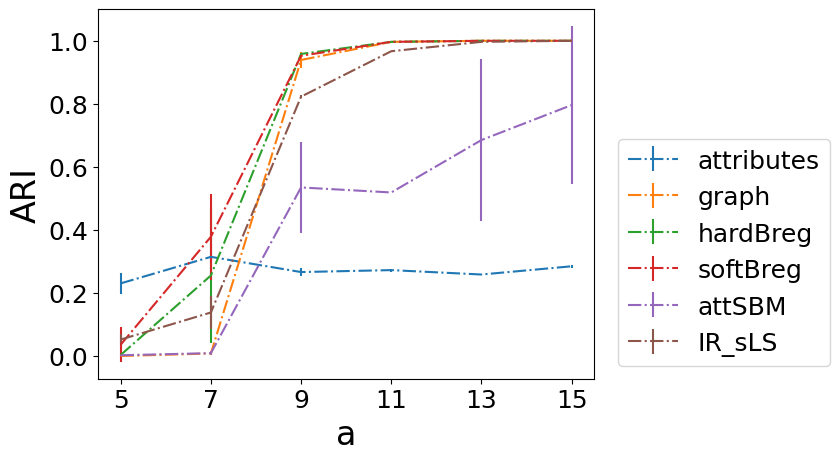
\includegraphics[width=\textwidth]{img/varying_a.png}
    \caption{Aumentando a informação da rede}
    \end{subfigure}
    \hfill
    \begin{subfigure}[b]{0.45\textwidth}
    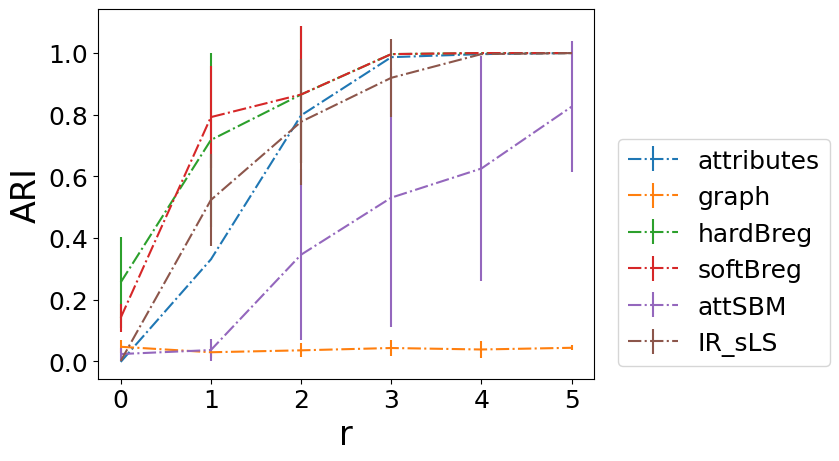
\includegraphics[width=\textwidth]{img/varying_r.png}
    \caption{Aumentando a informação dos atributos}
    \end{subfigure}
\end{figure}
\end{frame}



\begin{frame}{Robustez a Distribuição}
%    UM DOS INPUTS É A DISTRIBUIÇÃO UTILIZADA PARA GERAR OS DADOS. NO CENARIO REAL NOS NÃO SABEMOS A DISTRIBUIÇÃO A PRIORI. NOSSO ALGORITMO É ROBUSTO A ESSA SELEÇÃO. 

%% Deixar apenas o com atributos
%% MUDAR A LEGENDA PARA O RAIO
\begin{itemize}
	\item Um dos parâmetros é a distribuição dos dados
	\item Entretanto a metodologia é robusta nesse sentido, de não utilizar a distribuição exata
\end{itemize}
\begin{figure}
	\centering
	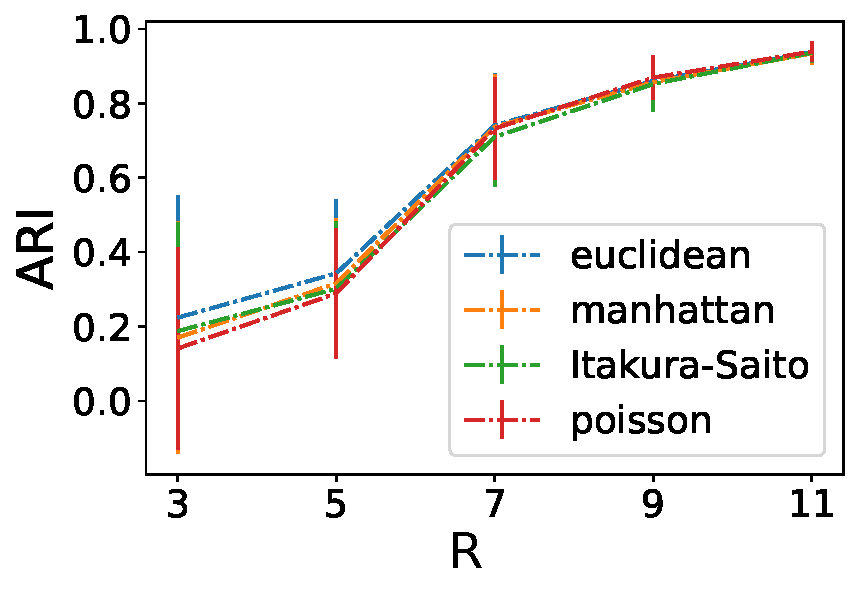
\includegraphics[scale=0.35]{img/varyingAttributeDivergence_netGaussian_attPoisson_N_200_K_2_pin_0,04_pout_0,01_muin_2_muout_0_nu2_3_nAverage_20.pdf}
	\caption{Várias divergências $d_{\psi^*}$. Poisson é o modelo correto.}
\end{figure}
\end{frame}


%% FALAR DE FORMA GERAL A DIVERSIDADE DOS DADOS
%% FALAR QUE NO PROX SLIDE OS DADOS FORAM PRE-PROCESSADOS PARA SE ADEQUAR A METODOLOGIA
\begin{frame}{Dados Reais}
\begin{itemize}
 \item \textbf{Cora}: $n=2708$, $m = 10556$, $d = 1433$, $K = 7$;
 \item \textbf{Citeseer}: $n = 3327$, $m = 9104$, $d = 3703$, $K=6 $; 
 \item \textbf{Wiscosin}: $n=251$, $m=515$, $d=1703$, $K=5$;
 \item \textbf{Texas}: $n=183$, $m=325$, $d=1703$, $K=5$;
 \item \textbf{Cornell}: $n=183$, $m=298$, $d=1703$, $K=5$;
\end{itemize}
n - Número de vértices;
m - Número de arestas;
d - Dimensão dos atributos;
K - Número de comunidades
\end{frame}

%% FALAR QUE NOSSOS RESULTADOS SÃO LIGEIRAMENTE MELHOR
\begin{frame}
	\begin{figure}
		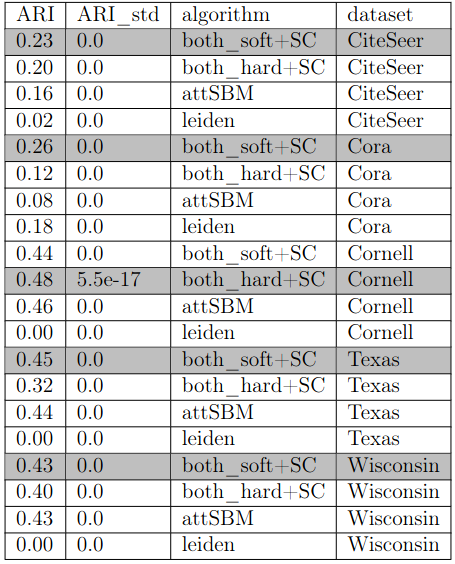
\includegraphics[scale=0.35]{img/comparison_table.png}
	\end{figure}

\end{frame}

\begin{frame}{Conclusão}
    \begin{itemize}
        \item Nosso método generaliza vários algoritmos permitindo qualquer distribuição exponencial a priori e grafos esparsos com pesos
        \item Discutimos novos métodos de inicialização
        \item Avaliações empíricas demonstram a superioridade do nosso modelo ao comparar com algoritmos competitivos 
        \item O método foi capaz de lidar bem com ambas as fontes de informação
        \item Artigo publicado na Neurips 2023
    \end{itemize}
\end{frame}

\begin{frame}
  \begin{figure}
  	\centering
  	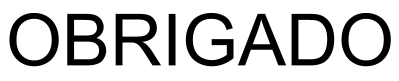
\includegraphics[scale=0.5]{img/OBRIGADO.png}
  \end{figure}
\end{frame}









\begin{frame}{Trabalhos futuros}
	\begin{itemize}
		\item Construir um algoritmo escalável, e comparar com outros benchmarks da literatura.
		\item Explorar outras divergências, de forma a generalizar para distribuições além da família exponencial, ex. t-student e Cauchy. 
		\item Métodos de inicialização mais eficientes
	\end{itemize}
\end{frame}

\begin{frame} {Formulação (Cont.)}
    \begin{itemize}
        \item Assumimos que as redes são esparsas, portanto: \begin{align*}
             f_{ab}(x) = (1-p_{ab}) \delta_0(x) + p_{ab} \fpos_{ab}(x), 
            \end{align*}
        \item Finalmente, assumimos que as distribuições $\{\fpos_{ab} \}$ e $\{h_a\}$ pertencem à família exponencial:
        \begin{align*}
        \label{eq:csbm_exponential_families}
         \fpos_{ab}(x) \weq e^{ <\theta_{ab}, x> - \psi(\theta_{ab}) } 
         \quad \text{ and } \quad
         h_a(y) \weq e^{<\eta_a, y> - \phi(\eta_a)}
        \end{align*}
        \item E.g. (gaussian): $\fpos _{ab}(x)  \weq e^{-\frac{(x-\mu_{ab})^2}{2\sigma^2}}$
    \end{itemize}
\end{frame}

%\begin{frame}{Exact Recovery Threshold}
%
%\begin{theorem}
%\label{thm:exact_recovery_CSBM}
% Consider model with $\pi_a > 0$ for all $a \in [K]$. Denote by $a^*, b^*$ the two hardest blocks to estimate, that is $\CH(a^*, b^*) = I$. 
% Suppose for all $t \in (0,1)$, $\lim\limits_{n \to \infty} \frac{n}{\log n} \CH_t(a^*,b^*)$ exists and is strictly concave. Then the following holds:
% \begin{enumerate}[(i)]
	%  \item exact recovery is information-theoretically impossible if 
	%  $\frac{n}{\log n} I < 1$;
	%  \item exact recovery is information-theoretically possible if 
	%  $\frac{n}{\log n} I > 1$. 
	% \end{enumerate}
%\end{theorem}
%\end{frame}

%\begin{frame}{Obtendo a Loglikelihood}
%
%\begin{itemize}
%    \item A fim de aplicar a propriedade da média como o minimizador, é conveniente minimizar a negativa da loglikelihood:  
%   \begin{align*}
	%         -\log \pr(X, Y \cond z) 
	%         & \weq \sum_{i} \left\{  \sum_{j \ne i} \left[ \dkl( A_{ij}, p_{z_i z_j}) + A_{ij} d_{\psi^*} \left( X_{ij}, \mu_{z_i z_j} \right) \right] + d_{\phi^*}(Y_i, \nu_{z_i}) \right\} + c
	%    \end{align*}
%    \item Para um único nó $i$ e comunidade $k$, e dada a matriz de pertencimento Z, a loglikelihood é:
%        \begin{align*}
	%             L_{ik}(Z) \weq \dkl \left( A_{i \cdot} , \left( Z p Z^T \right)_{i \cdot} \right) + A_{ij} d_{\psi^*} \left( X_{i \cdot} , \left( Z \mu Z^T \right)_{i \cdot} \right) + d_{\phi^*} \left( Y_i, \left( Z^T \nu \right)_i \right).
	%        \end{align*}
%    \end{itemize}
%\end{frame}

%\begin{frame}{Hard clustering}
%    \begin{figure}
%        \centering
%        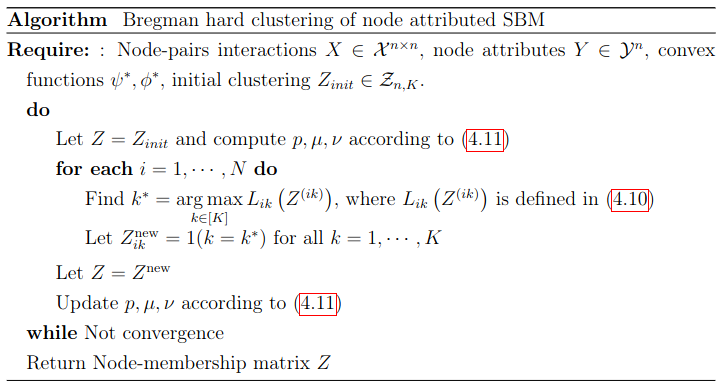
\includegraphics[scale=0.4]{img/hard_breg_sbm.png}
%    \end{figure}
%\end{frame}

\begin{frame}{Soft Clustering}
    Recall that ommiting the constants that depends on x we have:
    \begin{itemize}
        \item $f_{ab}(x) \weq \exp{\{ -\dkl(A_{ij}, p_{ab}) -A_{ij} d_{\psi^*}(X_{ij},\mu_{ab}) \} }$
        \item $h_{ab}(x) \weq \exp{\{ -d_{\phi^*}(x, \mu_{a})\}}$
    \end{itemize}
    Now we rewrite the Likelihood in the exponential form:
    {\small
    \begin{align*}  
        \pr \left( X,Y \cond z \right) & \weq \prod_{ 1\le i < j \le n } f_{z_i z_j}( X_{ij}) \prod_{i=1}^n h_{z_i} (Y_i)\\
         & \weq \exp{\{-\sum_{i,j}\left[ \dkl(A_{ij}, p_{z_i,z_j}) + A_{ij} d_{\psi^*}(X_{ij},\mu_{z_i,z_j})\right] - d_{\phi^*}(Y_i,\nu_{z_i}) \} }.
    \end{align*}
    }
\end{frame}

\begin{frame}{Update rule}
\begin{itemize}
    \item \textbf{E-step}:
        {\small
        \begin{align*}
            \tau_{ia} = p(z_i=a|X,Y, z_{-i}) & \propto p(X,Y| z_{-i}, z_i=a) p(z_i=a) \\
            & \propto \pi_a\exp{ \left\{ -\sum_{i,j}\left[\dkl(A_{ij}, p_{a,z_j}) + A_{ij} d_{\psi^*}(X_{ij},\mu_{a,z_j})\right] - d_{\phi^*}(Y_i,\nu_{a}) - c_i\right\} }
        \end{align*}
        }
    In practice, in order to have a stable exponent, we simply add a constant $c_i$ for every node:
    \begin{align*}
        c_i = \min_a \{\sum_{j}\left[ d_{net}(j)\right] + d_{\phi^*} (Y_i,\nu_{a})\}
    \end{align*}
    \item \textbf{M-step}:
        {\small
        \begin{align*}
         \hpi_k \weq \frac1n \sum_i \htau_{ik},
         \quad 
         \hmu_{k\ell} \weq \frac{ \sum_{i \ne j} \htau_{ik} \htau_{j\ell} X_{ij} }{ \sum_{i \ne j} \htau_{ik} \htau_{j \ell} }
         \quad \text{ and } \quad 
         \hnu_k \weq \frac{ \sum_i \htau_{ik} Y_{i} }{ \sum_i \htau_{ik} }. 
        \end{align*}
        }
\end{itemize}

\end{frame}

% \begin{frame}
	%     \begin{figure}
		%         \centering
		%     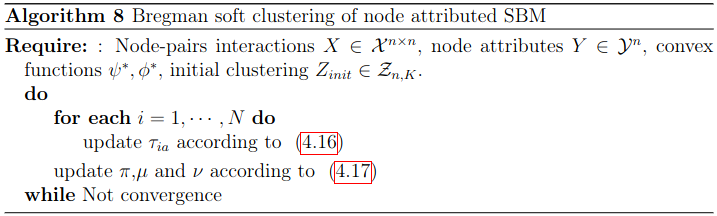
\includegraphics[scale=0.5]{img/soft_breg_sbm.png}
		%     \end{figure}
	% \end{frame}

\begin{frame}{Inicialização}
\hspace*{5px}
    Usamos a divergência de Chernoff-Hellinger para medir qual fonte dos dados nos dá maior informação:
        \begin{itemize}
	 \item Com $Z_{rede}$ para calcular:  
	 \begin{align*}
		     C_{rede}=\min\limits_{a\ne b} \sup\limits_{t \in (0,1)} (1-t) \sum\limits_{c=1}^K \pi_c \dren_t \left( f_{b c} \| f_{ac} \right)
		\end{align*}
	\item Com $Z_{atributos}$ para calcular:
	\begin{align*}
	 C_{atributos} = \min\limits_{a\ne b} \sup\limits_{t \in (0,1)} (1-t) \left[ \frac1n \dren_t \left( h_a \| h_b \right)\right]    
	 \end{align*}
	 \item Retornar $Z_{rede}$ se $C_{rede} > C_{atributos}$, do contrário retornar $Z_{atributos}$. 
	\end{itemize}
\end{frame}

\begin{frame}{Inicialização Espectral}
    \begin{enumerate}
	        \item Construir duas matrizes de similaridade, uma para os atributos e outra para a rede
	        \item Obter o Laplaciano
	        \item Computar os K menores autovetores de cada, deixando primeiro de fora
	        \item Concatenar os autovetores e agrupar no espaço projetado
	    \end{enumerate}
\end{frame}

\begin{frame}{Inicialização Espectral}
	\begin{figure}
		\centering
		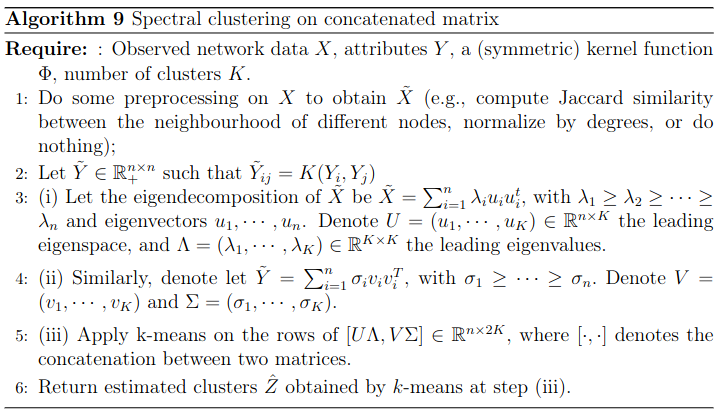
\includegraphics[scale=0.4]{img/spectral_init.png}
	\end{figure}
\end{frame}








 \begin{frame}
	     \begin{figure}[!ht]
		  \centering
		   \begin{subfigure}[b]{0.48\textwidth}
			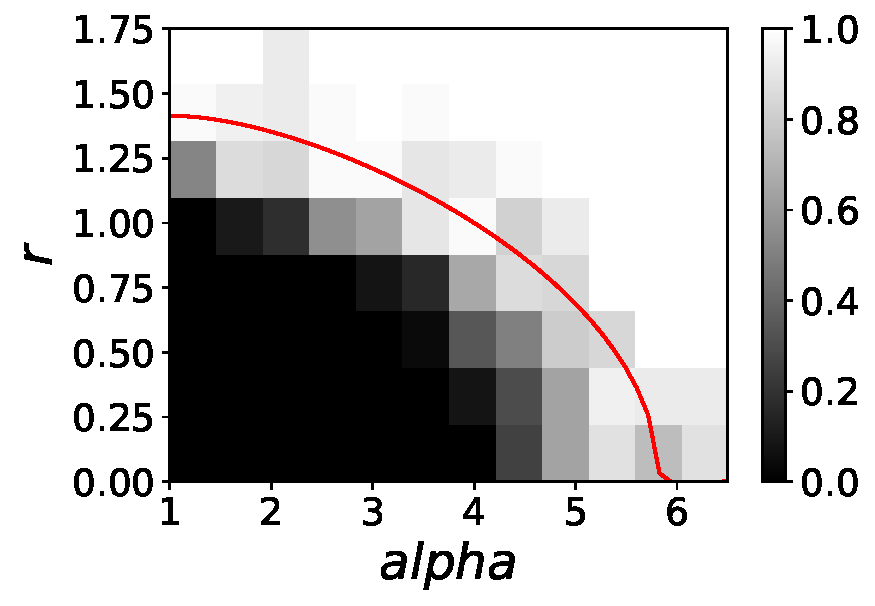
\includegraphics[width=\textwidth]{img/netBernoulli_attGaussian_beta_1_n_500_K_2_nAv_50_table8by10.pdf}
			\caption{Binary network with Gaussian attributes. Varying the $p_{in}$ and r.}
			\label{fig:information_theoretic_threshold_a}
			\end{subfigure}
		\hfill 
		\begin{subfigure}[b]{0.48\textwidth}
		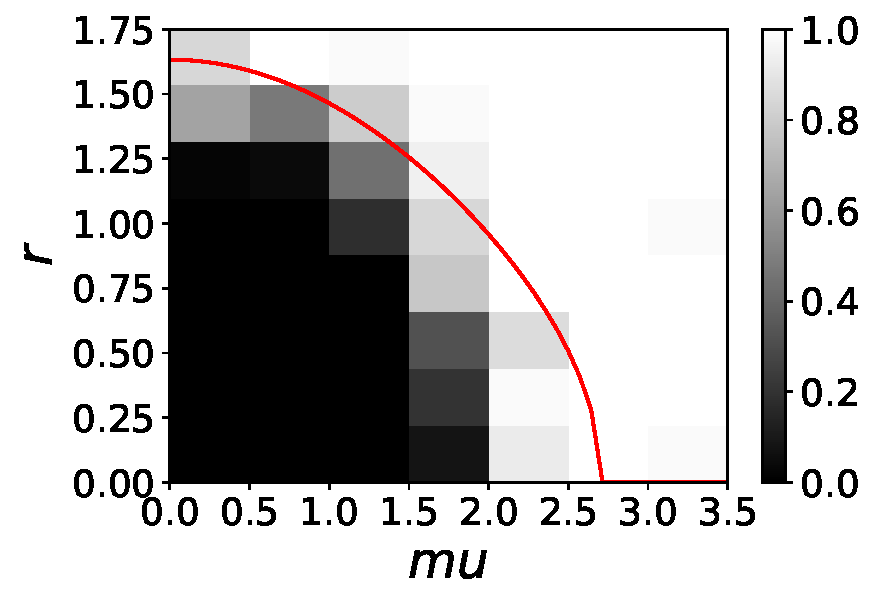
\includegraphics[width=\textwidth]{img/netGaussian0,mu_attGaussian_rho_5_n_600_K_3_nAv_50.pdf}
		\caption{zero-inflated Gaussian weights. We fix $w_{out} \sim \cN(0,1)$. Varying $w_{in} \sim \cN(\mu,1)$ and r}
		\label{fig:information_theoretic_threshold_b}
		 \end{subfigure}
		 \caption{Phase transition of exact recovery. Each pixel represents the empirical probability that Algorithm 1 succeeds at exactly recovering the clusters (over 50 runs), and the red curve shows the theoretical threshold.
		}
		\label{fig:information_theoretic_threshold}
		 \end{figure}
	\end{frame}



\begin{frame}{Resultados}
	%	FALAR DA SUPERIORIDADE DO ALGORITMO EM UM PONTO DO GRAFICO. MELHOR QUE SÓ REDE, SÓ ATRIBUTOS, E MELHOR QUE USAM AMBAS AS FONTES. FALAR A COR DE CADA LINHA TRACEJADA.
	
	%% Dizer que a curva azul não melhora pq utiliza apenas os atributos
	
	%% Dizer que a curva laranja não melhora pq utiliza apenas a rede


	\begin{figure}[!ht]
		\centering
		\begin{subfigure}[b]{0.3\textwidth}
			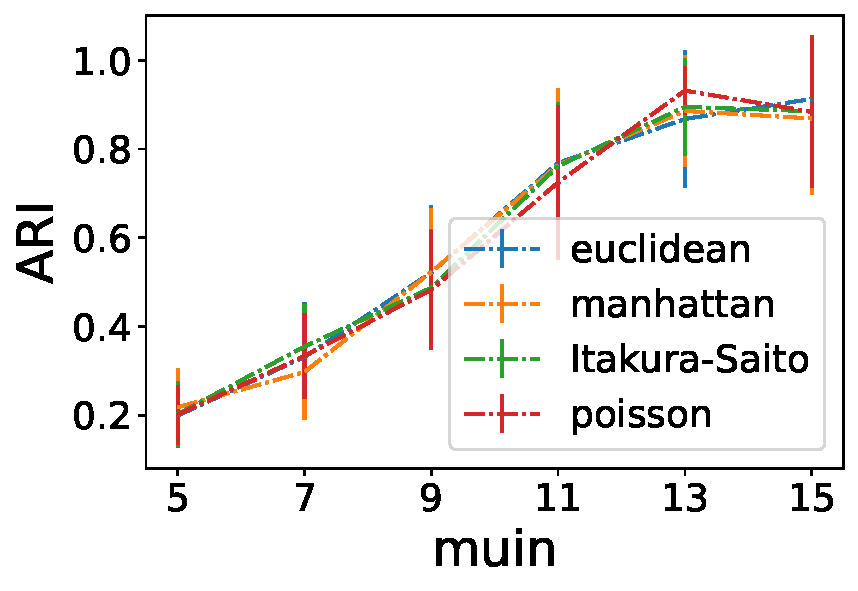
\includegraphics[width=\textwidth]{img/varyingNetworkDivergence_Poisson_Gaussian_N_400_K_4_pin_0,04_pout_0,01_muout_5_r_2_nAverage_20.pdf}
			\label{fig:varying_divergences_network}
		\end{subfigure}
		\hspace*{20px}
		\begin{subfigure}[b]{0.3\textwidth}
			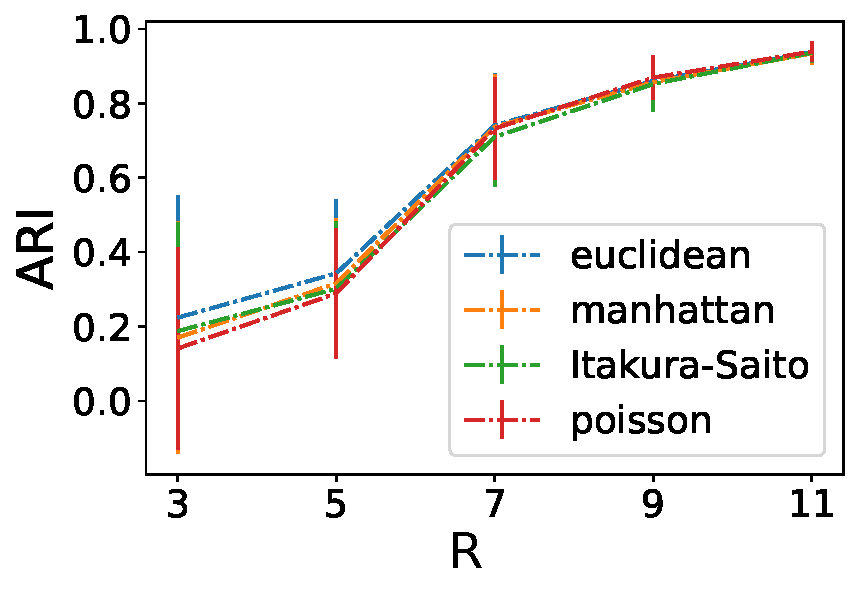
\includegraphics[width=\textwidth]{img/varyingAttributeDivergence_netGaussian_attPoisson_N_200_K_2_pin_0,04_pout_0,01_muin_2_muout_0_nu2_3_nAverage_20.pdf}
			\label{fig:varying_divergences_attributes}
		\end{subfigure}
		\caption{Adjusted Rand Index (ARI) averaged over 20 realisations \\
			(a) $n=400$, $k=4$, $\fin = (1-p)\delta_0(x) + p \mathrm{Poi}(\mu_{in})$ and $\fout = (1-q) \delta_0(x) + q \mathrm{Poi}(5)$, with $p=0.04$ and $q=0.01$. Attributes are 2d-Gaussians with unit variances and mean equally spaced the circle of radius $r=2$. \\ 
			(b) $n=400$, $k=2$, $\fin = (1-p)\delta_0(x) + p \mathrm{Nor}(2,1)$ and $\fout = (1-q) \delta_0(x) + q \mathrm{Nor}(0,1)$, with $p=0.04$ and $q=0.01$. Attributes are Poisson with means $\nu_1$ (for nodes in cluster 1) and $3$ (for nodes in cluster 2). 
		}
		\label{fig:varying_divergences}
	\end{figure}
\end{frame}



\begin{frame}{Resultados}
	%	FALAR DA SUPERIORIDADE DO ALGORITMO EM UM PONTO DO GRAFICO. MELHOR QUE SÓ REDE, SÓ ATRIBUTOS, E MELHOR QUE USAM AMBAS AS FONTES. FALAR A COR DE CADA LINHA TRACEJADA.
	
	%% Dizer que a curva azul não melhora pq utiliza apenas os atributos
	
	%% Dizer que a curva laranja não melhora pq utiliza apenas a rede
	\hspace*{10px}
	\begin{figure}[!ht]
		\centering
		\begin{subfigure}[b]{0.4\textwidth}
			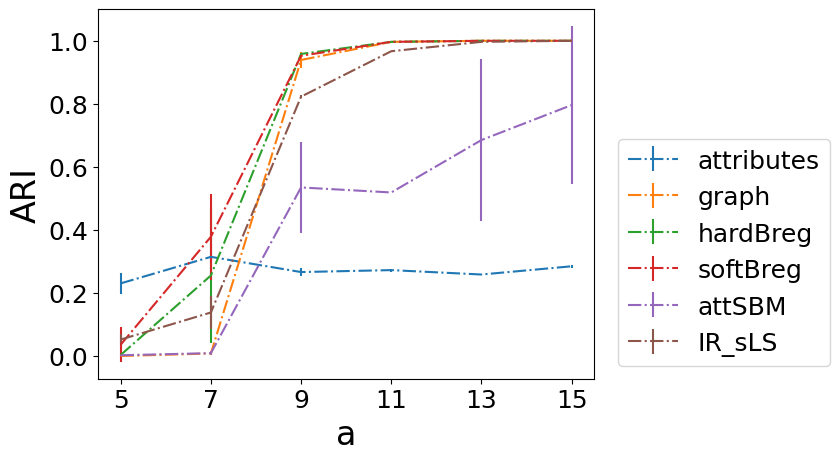
\includegraphics[width=\textwidth]{img/varying_a.png}
		\end{subfigure}
		\hfill
		\begin{subfigure}[b]{0.4\textwidth}
			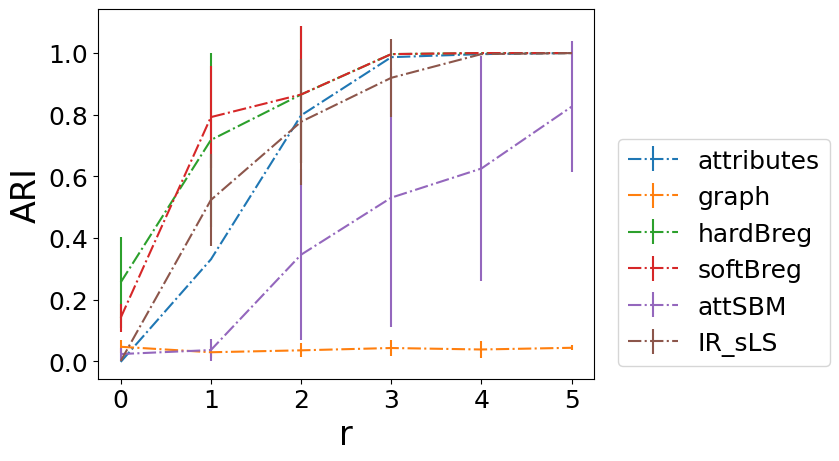
\includegraphics[width=\textwidth]{img/varying_r.png}
		\end{subfigure}
		    \caption{(a)Fixamos $p_{out} = 5 \frac{\log n}{n}$ e $r=1$. Variamos $p_{in} = a \frac{\log n}{n}$\\
			    (b) Fixamos $p_{out} = 5 \frac{\log n}{n}$, e $p_{in} = 8 \frac{\log n}{n}$. Variamos o raio R.\\ Ambos experimentos: atributos Gaussianos, grafo sem peso}
	\end{figure}
\end{frame}
%
% \begin{frame}{Attributed Stochastic Block Model \footnote{Stochastic Block Models with Multiple Continuous Attributes \cite{stanley2018stochastic} - Applied NetSci 2019}}
%    \begin{minipage}{.45\linewidth}
%        \begin{itemize}
%            \item Network and attributes are conditionally independent on the class labels:
%            \resizebox{.9 \textwidth}{!}
%            {
%                \begin{equation*}
%                {
%                \mathcal{L}_X = P(X|\Psi) = \sum_{i=1}^N\log\{\sum_{j=1}^K\pi_c\mathcal{N}(x_i|\mu_c,\Sigma_c)\}
%                 } 
%                \end{equation*}
%             }
%             \resizebox{.9 \textwidth}{!}
%            {
%                \begin{equation*}
%					
%                \mathcal{L}_A = \frac{1}{2}\sum_{i \ne j}\sum_{k,l}Z_{i,k}Z_{j,l} [a_{ij}\log{\theta_{kl}} + (1-a_{ij})\log(\theta_{kl})]
%					
%                \end{equation*}
%             }
%			
%			
%            \item Relies on expectation maximization procedure
%			
%        \end{itemize}
%    \end{minipage}    
%    \hfill
%     \begin{minipage}{0.45\textwidth}
%         \begin{figure}
%             \centering
%           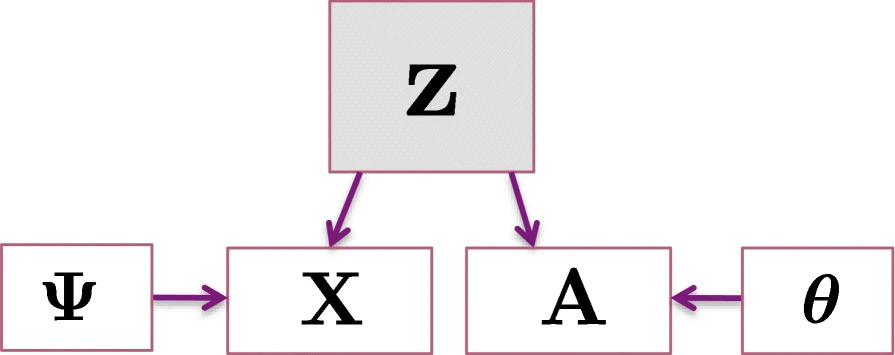
\includegraphics[scale=0.2]{img/PGM_attSBM.jpg}
%             \caption{A and X are assumed to be generated from a stochastic block model and a mixture of multivariate Gaussian distributions, parameterized by $\theta$ and $\Psi$, respectively.}
%         \end{figure}
%     \end{minipage}
%	
% \end{frame}



\begin{frame}{Contextual Stochastic Block Model \footnote{An iterative clustering algorithm for the Contextual Stochastic Block Model with optimality guarantees \cite{braun2022iterative} - ICML 2022}}
\begin{itemize}
     \item It also assumes Stochastic Block Model for the network and Gaussian Mixtures for the attributes.
     \item Doesn't rely on MLE.
     \item Optimization procedure is done via iterative refinement.
 \end{itemize}
\end{frame}

\begin{frame}
	
	\begin{table}
		\label{tab:other_metrics_real_data}
		
		\centering
		\npdecimalsign{.}
		\nprounddigits{2}
		\resizebox{0.5\columnwidth}{!}{%
			
			\begin{tabular}{|n{5}{2}|n{5}{2}|n{5}{2}|n{5}{2}|l|l|}
				\hline
				\text{S\&S} & \text{S\&S\_std} & \text{CC} & \text{CC\_std} & \text{algorithm} & \text{dataset} \\ \hline
				0.5300494085670995 & 0.003605798597739101 & 0.05800499648739317 & 0.006960312854227995 & both\_hard & CiteSeer \\ \hline
				0.6024645307639732 & 0.0 & 0.20451698681997663 & 0.0 & both\_hard+SC & CiteSeer \\ \hline
				0.5232144117101322 & 0.0036642837741560894 & 0.044840621275832326 & 0.0070770617339243795 & both\_soft & CiteSeer \\ \hline
				\rowcolor{Gray} 0.6193347299474888 & 0.0 & 0.23864739360285547 & 0.0 & both\_soft+SC & CiteSeer \\ \hline
				0.5501554634648966 & 0.0 & 0.0979837358951223 & 0.0 & kmeans & CiteSeer \\ \hline
				0.5355439242743328 & 0.0061474266091625105 & 0.06892920009476358 & 0.011922553299823752 & both\_hard & Cora \\ \hline
				0.5685312212956654 & 0.0 & 0.13404797824606526 & 0.0 & both\_hard+SC & Cora \\ \hline
				0.621415931227131 & 0.036859495152658135 & 0.24206236261735786 & 0.07387594997524789 & both\_soft & Cora \\ \hline
				\rowcolor{Gray} 0.6314235770136144 & 0.0 & 0.26231353709828864 & 0.0 & both\_soft+SC & Cora \\ \hline
				0.5261459359896783 & 0.0 & 0.05068206132120533 & 6.938893903907228e-18 & kmeans & Cora \\ \hline
				0.5136161379431157 & 0.004658523136779102 & 0.02718712041475387 & 0.00929508769009895 & both\_hard & Cornell \\ \hline
				\rowcolor{Gray} 0.7511393439872041 & 0.0 & 0.5009025617377737 & 0.0 & both\_hard+SC & Cornell \\ \hline
				0.5380532572495016 & 0.022333799112504136 & 0.07584356889568729 & 0.044411102162164914 & both\_soft & Cornell \\ \hline
				0.7309438319978814 & 0.0 & 0.46036991971585256 & 0.0 & both\_soft+SC & Cornell \\ \hline
				0.6823871791537457 & 0.0 & 0.3628568888150612 & 0.0 & kmeans & Cornell \\ \hline 
				0.5707435162291284 & 0.03546092916435076 & 0.14076723826311163 & 0.07054592332122592 & both\_hard & Texas \\ \hline
				0.6649669857624094 & 0.0 & 0.32953213859345204 & 0.0 & both\_hard+SC & Texas \\ \hline
				0.6692402403185131 & 0.037481321156439984 & 0.33832138613528306 & 0.07484925023694196 & both\_soft & Texas \\ \hline
				0.7271925640211407 & 0.0 & 0.4542508823527238 & 0.0 & both\_soft+SC & Texas \\ \hline
				\rowcolor{Gray} 0.7424955998664785 & 0.0 & 0.4847729373333235 & 5.551115123125783e-17 & kmeans & Texas \\ \hline
				0.5809942156514938 & 0.016798869015950336 & 0.16085140140659873 & 0.03348483159124113 & both\_hard & Wisconsin \\ \hline
				0.7006960666909214 & 0.0 & 0.40126208623137005 & 0.0 & both\_hard+SC & Wisconsin \\ \hline
				0.6395089689635596 & 0.01183809504444334 & 0.27884136012871213 & 0.023627897675137528 & both\_soft & Wisconsin \\ \hline
				\rowcolor{Gray} 0.7199863595576359 & 0.0 & 0.4388325192714809 & 5.551115123125783e-17 & both\_soft+SC & Wisconsin \\ \hline
				0.6868962279261217 & 0.0 & 0.37346426015369016 & 0.0 & kmeans & Wisconsin \\ \hline
			\end{tabular}
			\npnoround
		}
	\end{table}
\end{frame}
\end{document}

